\section{Results}
\label{sec:results}

% Figure ordering: the user-suggested layout puts the efficiency Pareto
% plot as the headline figure (Fig. 1), since it encapsulates the
% strongest message in one image. Architecture diagram follows as
% Fig. 2.

\subsection{The DPA4 architecture}
\label{sec:arch_overview}

DPA4 was designed as a conservative equivariant potential in which the main
geometric work is shared across all interaction blocks
(Fig.~\ref{fig:arch}a,b). For each neighbour graph, the model constructs a
single edge cache containing smooth cutoff envelopes, radial-species features,
local gauges and short-range bridging gates. The same cache feeds the input
embedding, the SO(2) interaction blocks and the analytical ZBL branch. This
organization avoids repeated geometry construction while ensuring that
energies, forces and virials are all derived from one scalar potential.

The central architectural choice is to perform equivariant message passing in
an edge-local SO(2) representation rather than through full SO(3)
Clebsch--Gordan tensor products (Fig.~\ref{fig:arch}c). Aligning each bond with
a local reference axis reduces the residual symmetry of the edge update to
SO(2), so coefficients can be processed in fixed $|m|$ strata. Within these
strata, DPA4 uses edge-conditioned radial degree coupling and multi-focus SO(2)
convolutions to mix angular degrees without introducing a separate equivariant
edge feature. The construction retains the directional representation needed
for equivariant molecular and materials modelling while reducing the algebraic
cost of each message update.

Two additional components make this local-frame architecture effective in the
benchmarks below. First, the Environment Initial Embedding supplies the scalar
backbone with a rotation-invariant local-environment prior at layer 0, while
the higher-degree initial features carry directional information from spherical
harmonics. Second, envelope-gated softmax attention aggregates edge messages
with invariant weights that vanish smoothly at the cutoff. The attention
mechanism therefore increases the flexibility of neighbourhood aggregation
without breaking equivariance or introducing a discontinuity in the
conservative energy.

DPA4 also treats short-range nuclear repulsion as part of the model rather than
as an external correction. The analytical ZBL energy is summed with the neural
branch before differentiation, and Native ZBL Zone Bridging removes the direct
learned short-range pair channel in the inner frozen zone. Thus the model keeps
the differentiable scalar-energy formulation used for force training while
assigning the singular short-range pair interaction to a physically motivated
analytical branch.

The architecture is co-designed with the training system. Conservative MLIP
training is difficult to compile because the force loss differentiates through
$\mathbf{F}=-\partial E/\partial R$ and therefore requires mixed
coordinate--parameter second derivatives. DPA4 removes this barrier by tracing
the energy-to-force derivative into an ordinary tensor graph and lowering the
resulting conservative-force path with \texttt{torch.compile}. This makes the
same scalar-energy model trainable in compiled mode rather than switching to a
direct-force surrogate, and is the main source of the 2--3$\times$ wall-clock
training speedup quantified below. The optimiser is matched to this structure:
HybridMuon applies matrix-aware Muon updates to hidden transformations, keeps
scalar and normalisation parameters on Adam-family updates, and updates
degree-indexed equivariant tensors in slice mode so that distinct SO(2)
representation blocks are not flattened into one unrelated matrix.

\begin{figure}[t]
    \centering
    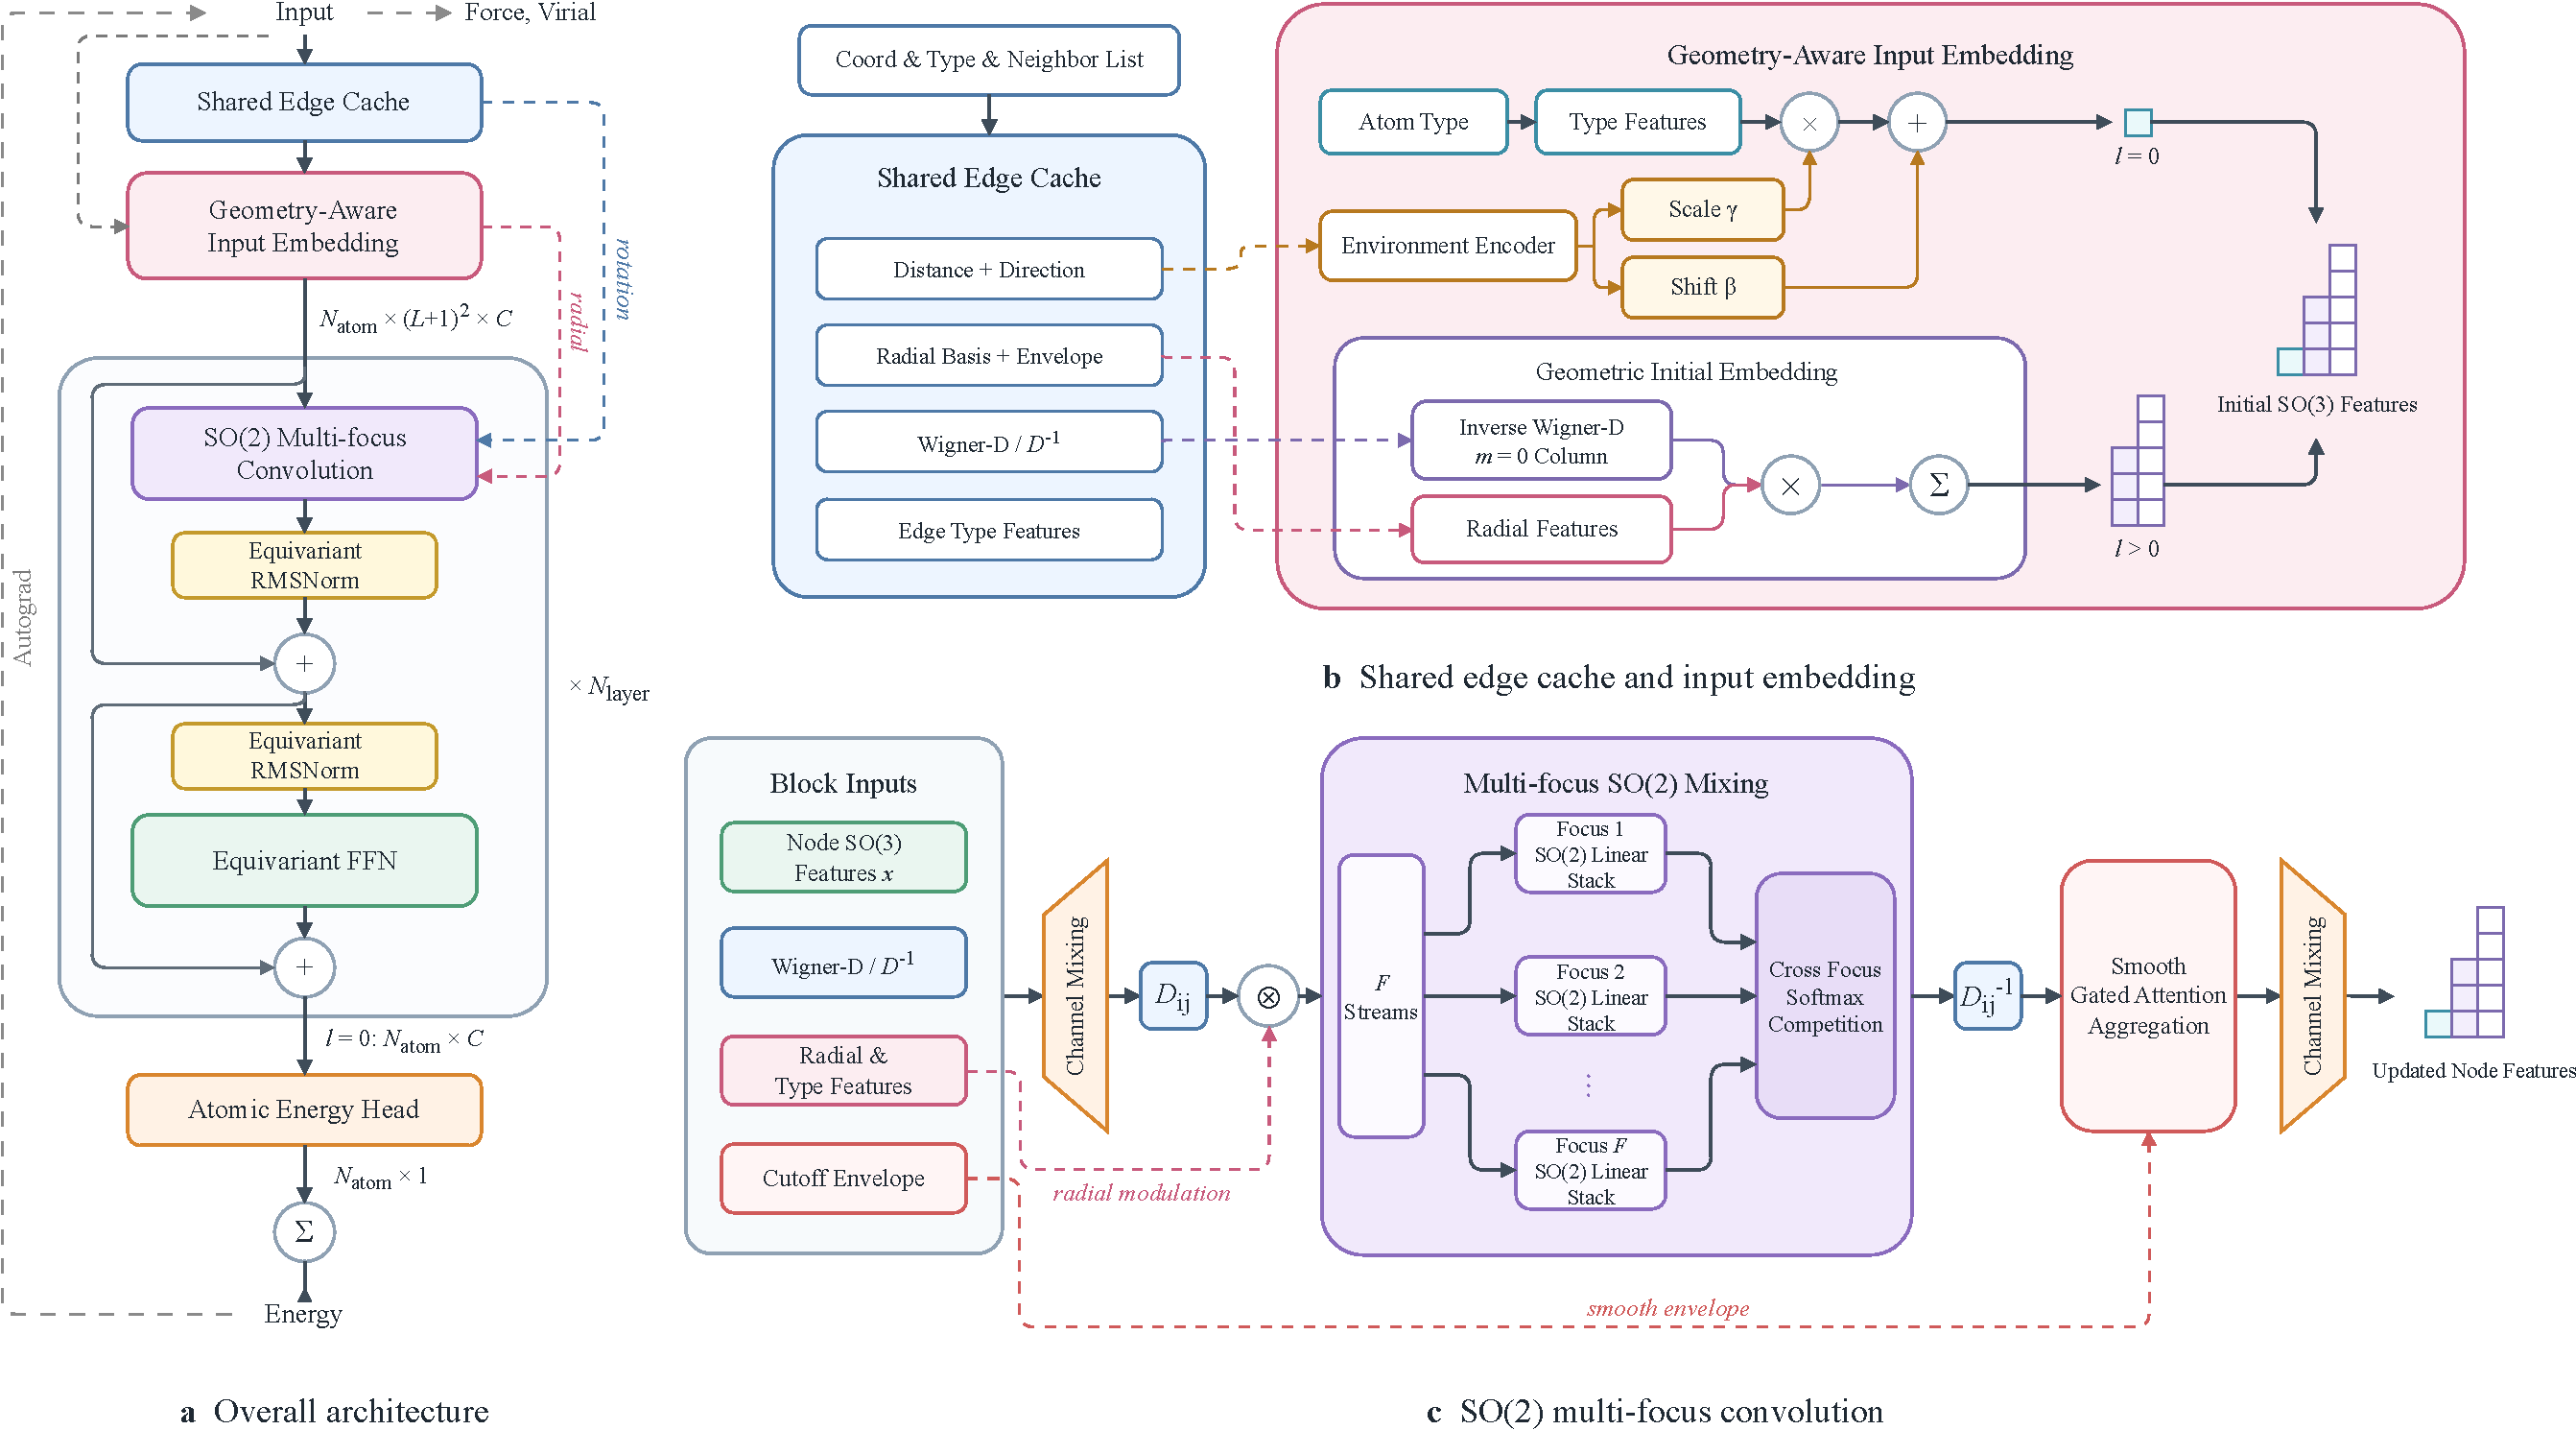
\includegraphics[width=\textwidth]{fig/fig2_simplified.pdf}
    \caption{
        Overview of the DPA4 architecture.
        (a) The full model combines a shared edge cache, geometry-aware input
        embedding, stacked equivariant interaction blocks, and an atomic energy
        head.
        (b) Geometry and radial features are computed once and reused by the input
        embedding and all interaction blocks.
        (c) Each SO(2) multi-focus convolution rotates features to an edge-local
        frame, applies radial modulation and focus competition, and aggregates
        messages after rotating them back.
    }
    \label{fig:arch}
\end{figure}

\subsection{Matbench Discovery}
\label{sec:matbench}

\begin{table}
    \centering
    \caption{Results on the Matbench Discovery leaderboard, with all compliant models accessed before May 25, 2026.}
    \label{tab:matbench}

    \resizebox{\linewidth}{!}{
        \begin{tabular}{@{} l *{9}{c} c c @{}}
            \toprule
            \textbf{Model}       & \textbf{CPS}$\uparrow$ & \textbf{Acc}$\uparrow$ & \textbf{F1}$\uparrow$ & \textbf{DAF}$\uparrow$ & \textbf{Prec}$\uparrow$ & \textbf{MAE}$\downarrow$ & \textbf{R2}$\uparrow$ & \textbf{$\kappa$SRME}$\downarrow$ & \textbf{RMSD}$\downarrow$ & \textbf{Params}$\downarrow$ & \textbf{Targets} \\
            \midrule
            DPA4-Pro             &                        &                        &                       &                        &                         &                          &                       &                                   &                           &                             &                  \\
            DPA4-Plus            &                        &                        &                       &                        &                         &                          &                       &                                   &                           &                             &                  \\
            DPA4                 &                        &                        &                       &                        &                         &                          &                       &                                   &                           &                             &                  \\
            DPA4-Air             & 0.804                  & 0.946                  & 0.828                 & 5.303                  & 0.811                   & 0.035                    & 0.743                 & 0.302                             & 0.075                     & 2.76M                       & EFSG             \\
            DPA4-Neo             & 0.781                  & 0.941                  & 0.815                 & 5.189                  & 0.793                   & 0.036                    & 0.805                 & 0.367                             & 0.079                     & 1.60M                       & EFSG             \\
            \midrule
            EquiformerV3+DeNS-MP & 0.830                  & 0.956                  & 0.863                 & 5.479                  & 0.838                   & 0.029                    & 0.840                 & 0.275                             & 0.070                     & 30.3M                       & EFSG             \\
            eSEN-30M-MP          & 0.797                  & 0.946                  & 0.831                 & 5.260                  & 0.804                   & 0.033                    & 0.822                 & 0.340                             & 0.075                     & 30.1M                       & EFSG             \\
            MatRIS-10M-MP        & 0.778                  & 0.951                  & 0.847                 & 5.422                  & 0.829                   & 0.031                    & 0.824                 & 0.489                             & 0.072                     & 10.4M                       & EFSGM            \\
            Eqnorm MPtrj         & 0.756                  & 0.929                  & 0.786                 & 4.844                  & 0.741                   & 0.040                    & 0.799                 & 0.408                             & 0.084                     & 1.31M                       & EFSG             \\
            Nequix MP PFT        & 0.755                  & 0.914                  & 0.748                 & 4.479                  & 0.685                   & 0.044                    & 0.784                 & 0.307                             & 0.087                     & 708k                        & EFSHG            \\
            Nequip-MP-L          & 0.733                  & 0.921                  & 0.761                 & 4.704                  & 0.719                   & 0.043                    & 0.791                 & 0.452                             & 0.086                     & 9.6M                        & EFSG             \\
            Nequix MP            & 0.729                  & 0.914                  & 0.751                 & 4.455                  & 0.681                   & 0.044                    & 0.782                 & 0.446                             & 0.085                     & 708k                        & EFSG             \\
            Allegro-MP-L         & 0.720                  & 0.915                  & 0.751                 & 4.516                  & 0.690                   & 0.044                    & 0.778                 & 0.504                             & 0.082                     & 18.7M                       & EFSG             \\
            DPA-3.1-MPtrj        & 0.718                  & 0.936                  & 0.803                 & 5.024                  & 0.768                   & 0.037                    & 0.812                 & 0.650                             & 0.080                     & 4.81M                       & EFSG             \\
            SevenNet-l3i5        & 0.714                  & 0.920                  & 0.760                 & 4.629                  & 0.708                   & 0.044                    & 0.776                 & 0.550                             & 0.085                     & 1.17M                       & EFSG             \\
            HIENet               & 0.707                  & 0.929                  & 0.777                 & 4.932                  & 0.754                   & 0.041                    & 0.793                 & 0.642                             & 0.080                     & 7.51M                       & EFSG             \\
            GRACE-2L-MPtrj       & 0.681                  & 0.895                  & 0.691                 & 4.163                  & 0.636                   & 0.052                    & 0.741                 & 0.526                             & 0.090                     & 15.3M                       & EFSG             \\
            MACE-MP-0            & 0.637                  & 0.878                  & 0.669                 & 3.777                  & 0.577                   & 0.057                    & 0.697                 & 0.682                             & 0.092                     & 4.69M                       & EFSG             \\
            eqV2 S DeNS          & 0.522                  & 0.939                  & 0.815                 & 5.042                  & 0.771                   & 0.036                    & 0.788                 & 1.676                             & 0.076                     & 31.2M                       & EFSD             \\
            ORB v2 MPtrj         & 0.470                  & 0.922                  & 0.765                 & 4.702                  & 0.719                   & 0.045                    & 0.756                 & 1.726                             & 0.101                     & 25.2M                       & EFSD             \\
            CHGNet               & 0.343                  & 0.851                  & 0.613                 & 3.361                  & 0.514                   & 0.063                    & 0.689                 & 2.000                             & 0.095                     & 413k                        & EFSGM            \\
            M3GNet               & 0.310                  & 0.812                  & 0.569                 & 2.882                  & 0.441                   & 0.075                    & 0.585                 & 2.000                             & 0.112                     & 228k                        & EFSG             \\
            \bottomrule
        \end{tabular}%
    }
\end{table}

Matbench Discovery evaluates the ability of machine-learning interatomic
potentials to support high-throughput inorganic-crystal discovery. Following
the compliant leaderboard protocol, models trained on MPtrj are used to relax
WBM candidate structures and predict their formation energies; these predictions
are converted into convex-hull distances and assessed by classification,
regression and structural-relaxation metrics. Table~\ref{tab:matbench} compares
DPA4 with representative compliant models under this protocol.

The largest evaluated model, DPA4-Pro, establishes a new state-of-the-art point
on this benchmark, reaching a CPS of 0.830, an F1 score of 0.850 and a
$\kappa$SRME of 0.241 with 32.7M parameters. The compact DPA4 variants occupy a
strong accuracy--efficiency regime. DPA4-Air reaches a CPS of 0.804, exceeding
eSEN-30M-MP while using 2.76M rather than 30.1M parameters. Its WBM energy MAE
is 0.035~eV/atom, close to eSEN-30M-MP, and its $\kappa$SRME is lower
(0.302 versus 0.340), indicating that the gain is not obtained by sacrificing
relaxation quality. The smaller DPA4-Neo model, with only 1.60M parameters,
still reaches a CPS of 0.781, comparable to MatRIS-10M-MP and above most
published compliant baselines. These results show that the local-frame SO(2)
architecture can deliver state-of-the-art crystal-discovery accuracy while also
scaling down to substantially smaller models.

\subsection{Small-molecule benchmarks}
\label{sec:small_mol}

We next evaluate DPA4 on SPICE-MACE-OFF, the organic-molecule benchmark used by
MACE-OFF. The benchmark contains PubChem molecules, DES370K monomers and
dimers, dipeptides, solvated amino acids, water clusters and QMugs-derived
larger molecules, with reference energies and forces computed at the
$\omega$B97M-D3(BJ)/def2-TZVPPD level. We keep the train/validation/test split
used in the MACE-OFF and DPA3 comparisons and report per-subset energy and
force MAEs together with a logarithmic weighted average MAE (LWAMAE), which
summarizes performance across chemically heterogeneous subsets without allowing
one high-error subset to dominate the aggregate score.

\begin{table}
    \scriptsize
    \caption{Test MAE on SPICE-MACE-OFF dataset. Energy (E) MAE is in meV/atom and force (F) MAE is in meV/\AA.}
    \label{table:spice}
    \centering
    \begin{threeparttable}
        \begin{spacing}{1.15}
            \begin{tabular}{l
                    | R{0.55cm}R{0.55cm}  % MACE(M)
                    | R{0.55cm}R{0.55cm}  % MACE(L)
                    | R{0.55cm}R{0.55cm}  % eSEN (3.2M)
                    | R{0.55cm}R{0.55cm}  % eSEN (6.5M)
                    | R{0.55cm}R{0.55cm}  % DPA3-L24
                    | R{0.55cm}R{0.55cm}  % DPA4: Air
                    | R{0.55cm}R{0.55cm}  % DPA4: Plus
                }
                \toprule
                                   & \multicolumn{2}{c|}{MACE(M)} & \multicolumn{2}{c|}{MACE(L)} & \multicolumn{2}{c|}{eSEN}  & \multicolumn{2}{c|}{eSEN}  & \multicolumn{2}{c|}{DPA3-L24} & \multicolumn{2}{c|}{DPA4: Air} & \multicolumn{2}{c}{DPA4: Plus}                                                                                                                          \\\hline
                \textbf{Dataset}   & \textbf{E~~~}                & \textbf{F~~~}                & \textbf{E~~~}              & \textbf{F~~~}              & \textbf{E~~~}                 & \textbf{F~~~}                  & \textbf{E~~~}                  & \textbf{F~~~}    & \textbf{E~~~} & \textbf{F~~~} & \textbf{E~~~}    & \textbf{F~~~}    & \textbf{E~~~} & \textbf{F~~~} \\
                PubChem            & 0.91                         & 20.57                        & 0.88                       & 14.75                      & 0.22                          & 6.10                           & \underline{0.15}               & 4.21             & 0.24          & 8.47          & 0.16             & \underline{4.15} & \textbf{0.12} & \textbf{3.21} \\
                DES370K M.         & 0.63                         & 9.36                         & 0.59                       & 6.58                       & 0.17                          & 1.85                           & \underline{0.13}               & \underline{1.24} & 0.18          & 3.15          & 0.15             & 1.37             & \textbf{0.12} & \textbf{0.98} \\
                DES370K D.         & 0.58                         & 9.02                         & 0.54                       & 6.62                       & 0.20                          & 2.77                           & 0.15                           & 2.12             & 0.23          & 3.19          & \underline{0.12} & \underline{1.38} & \textbf{0.09} & \textbf{0.98} \\
                Dipeptides         & 0.52                         & 14.27                        & 0.42                       & 10.19                      & 0.10                          & 3.04                           & 0.07                           & 2.00             & 0.13          & 4.81          & \underline{0.06} & \underline{1.98} & \textbf{0.04} & \textbf{1.39} \\
                Sol. AA            & 1.21                         & 23.26                        & 0.98                       & 19.43                      & 0.30                          & 5.76                           & 0.25                           & \underline{3.68} & 0.31          & 8.77          & \underline{0.17} & 3.77             & \textbf{0.11} & \textbf{2.75} \\
                Water              & 0.76                         & 15.27                        & 0.83                       & 13.57                      & 0.24                          & 3.88                           & 0.15                           & \underline{2.50} & 0.32          & 6.89          & \underline{0.11} & 2.52             & \textbf{0.09} & \textbf{1.89} \\
                QMugs              & 0.69                         & 23.58                        & 0.54                       & 16.93                      & 0.16                          & 5.70                           & 0.12                           & 3.78             & 0.17          & 8.66          & \underline{0.08} & \underline{3.52} & \textbf{0.06} & \textbf{2.47} \\\hline
                LWAMAE\tnote{a}    & 0.73                         & 15.42                        & 0.65                       & 11.66                      & 0.19                          & 3.83                           & 0.14                           & 2.58             & 0.22          & 5.78          & \underline{0.12} & \underline{2.44} & \textbf{0.09} & \textbf{1.77} \\\hline
                \textbf{\# Params} & \multicolumn{2}{c|}{2.3 M}   & \multicolumn{2}{c|}{6.9 M}   & \multicolumn{2}{c|}{3.2 M} & \multicolumn{2}{c|}{6.5 M} & \multicolumn{2}{c|}{4.9 M}    & \multicolumn{2}{c|}{2.7 M}     & \multicolumn{2}{c}{5.3 M}                                                                                                                               \\
                \toprule
            \end{tabular}
            \begin{tablenotes}
                \item[a] \footnotesize The Logarithmic Weighted Average MAE is the exponential of the unweighted mean of logarithmic subset MAEs.
            \end{tablenotes}
        \end{spacing}
    \end{threeparttable}
\end{table}

Table~\ref{table:spice} shows that DPA4 improves the molecular benchmark
accuracy consistently across all subsets. DPA4-Plus gives the lowest energy and
force MAEs in every subset and reduces the aggregate LWAMAE to
0.09~meV/atom for energies and 1.77~meV/\AA{} for forces. Relative to the
6.5M-parameter eSEN baseline, this corresponds to approximately 36\% lower
energy LWAMAE and 31\% lower force LWAMAE with a smaller 5.3M-parameter model.
Relative to DPA3-L24, the reductions are approximately 59\% and 69\%,
respectively, indicating that the gain is not limited to inorganic crystals.

The smaller DPA4-Air model also performs competitively. With 2.7M parameters, it
already improves upon the 6.5M-parameter eSEN model in aggregate energy and
force LWAMAEs and is second-best in most subset-level comparisons. The
improvement is especially pronounced for water, solvated amino acids and QMugs,
where DPA4-Air substantially lowers the energy error relative to DPA3-L24 while
remaining close to the larger DPA4-Plus model. Together, the two DPA4 sizes show
that the SO(2) attention architecture transfers from inorganic crystals to
organic molecules and offers a favourable accuracy--parameter trade-off across
chemically diverse data.

\subsection{Training and inference efficiency}
\label{sec:efficiency}

% This subsection carries the strongest single message. Lead with the
% Pareto figure.

% TODO: Fig. 1 --- the headline Pareto plot.
%   - x-axis: cumulative GPU-hours (or wall-clock training time), log scale
%   - y-axis: WBM energy MAE (Matbench Discovery test), log scale
%   - Plot every Matbench-Discovery-compliant model for which training
%     trajectories are available (CHGNet, M3GNet, MACE-MP-0, SevenNet,
%     GRACE, AlphaNet, MatRIS, eSEN-30M-MP, ORB, eqV2, DPA3-L24, ...).
%   - Highlight DPA4 as a new Pareto frontier strictly below and to
%     the left of all baselines.
%   - This figure can also serve as the visual abstract.

% TODO: Tab. 2 --- training & inference efficiency details.
%   Rows: DPA3-L24, DPA4-L24, DPA4-L24 (no compile), MACE(L), eSEN.
%   Columns:
%     - # parameters
%     - Training throughput (samples / s)
%     - GPU-hours to reach target WBM MAE = [TODO: X] meV/atom
%     - ASE single-point latency at 80 / 200 / 500 / 1000 / 5000 atoms (ms)
%     - Peak GPU memory (GB) at fixed batch size

% TODO: write 3 short paragraphs.

% ¶1 --- Algorithmic efficiency.
%   - SO(2) ops are diagonal in the angular-order basis: O(d * m_max)
%     per edge, vs SO(3) Clebsch--Gordan products that scale as O(L^6)
%     in the maximum spherical-harmonic order.
%   - Report FLOPs ratio of DPA4's edge update vs a comparable
%     MACE-style SO(3) model.

% ¶2 --- Implementation efficiency (torch.compile).
%   - Why traditional MLIPs (incl. DPA3) cannot be torch.compile'd
%     cleanly: dynamic neighbor counts, in-place graph buffers, Python
%     control flow on the hot path, custom CUDA kernels with no
%     dispatcher coverage.
%   - DPA4's redesign: padded-neighbor representation, functional
%     (non-in-place) updates, use of torch.fx / make_fx-style tracing
%     where appropriate, plus full dispatcher coverage on hot ops.
%   - Report compile-time overhead and steady-state speedup from
%     enabling torch.compile alone (i.e. with/without compile on
%     identical model + hardware).

% ¶3 --- End-to-end claim and hardware portability.
%   - Headline: at matched WBM MAE, DPA4 reaches the target in
%     [TODO: 5--10x] fewer GPU-hours and uses [TODO: X%] of DPA3's
%     peak memory.
%   - Inference at large system size (5000 atoms): [TODO: Yx] faster
%     than DPA3-L24, [TODO: Zx] faster than MACE(L).
%   - Portability: report training throughput on V100 and RTX 4090
%     (in addition to A800) to demonstrate that DPA4 is usable on
%     commodity GPUs, not just data-center accelerators.

\subsection{Native ZBL coupling and extreme conditions}
\label{sec:zbl}

% TODO: Fig. 4(a) --- short-range energy curve.
%   - For one or two atom pairs, plot the combined pair energy vs r,
%     showing the smooth crossover from NN to ZBL.
%   - Annotate r_in and r_out, and verify C^2 continuity visually.

% TODO: Fig. 4(b) --- cascade case study.
%   - Pick the simplest example with a clear DPA4-ZBL vs DPA4-noZBL gap.
%   - Suggested: PKA cascade in W (well-known irradiation benchmark).
%   - Plot total energy drift / atomic-displacement stability vs
%     simulation time; show DPA4-noZBL diverging while DPA4-ZBL stays
%     stable.
%   - Optional: overlay DPA3-with-external-ZBL or MACE-MP-0-with-ZBL
%     to show that wrapper-style ZBL breaks conservativeness on a
%     measurable timescale.

% TODO: write 1--2 paragraphs.
%
% ¶1 --- Why wrapper-style ZBL is not enough.
%   Briefly recap how DPA3-style or MACE-MP-0-style ZBL is applied
%   externally and why this can break C^2 smoothness or
%   conservativeness.
%
% ¶2 --- DPA4's native coupling and impact.
%   Smooth switch is applied per pair before energy summation; forces
%   and virials remain conservative by construction. Use the case
%   study to illustrate practical impact (high-energy collisions,
%   compression/melting, rare close-distance configurations on
%   reaction paths).

\subsection{Architecture ablations}
\label{sec:ablation}

We evaluate the main architectural and implementation choices of DPA4 on the
same WBM-subsampled test set and report energy and force MAEs under a shared
evaluation protocol. Because the ablations isolate different factors only
within their own controlled groups, each group is interpreted as evidence for
the corresponding design choice rather than as part of a global ranking across
unrelated runs. Efficiency metrics are reported as relative quantities under
matched hardware, batch-size, data-loading, and precision settings. Unless
otherwise noted, \textit{Train time (rel.)} denotes relative training
wall-clock time, and \textit{Test time (rel.)} denotes the relative wall-clock
time required to evaluate the full WBM-subsampled test set with the DeePMD-kit
\texttt{dp test} command. Although the test set and hardware are matched, test
time is retained as a secondary throughput reference because model size changes
the feasible batch size, memory pressure, and kernel execution pattern.
Normalized training time is therefore the primary efficiency metric. In tables
where rank highlighting is used, boldface denotes the best value within the
corresponding controlled comparison and underlining denotes the second-best
value. We omit second-best underlining for metrics without an explicitly
highlighted best value or when multiple rows are tied for the best value.

\subsubsection{Compilation and training precision}

This ablation tests the effect of enabling \texttt{torch.compile} together with
the training-precision choices used by DPA4. We separate three factors: graph
compilation, bfloat16 automatic mixed precision (AMP), and TF32 tensor-core
matmul. As a graph-level execution transformation, \texttt{torch.compile} does
not change the model equations; correspondingly, the reported compiled
configurations do not show a visible accuracy loss attributable to compilation.
Table~\ref{tab:dpa4_compile_ablation} shows that bf16 AMP reduces the training
time by approximately 30\% and peak training memory by approximately 59\%
relative to the non-compiled FP32 baseline. In the compiled setting, bf16 AMP
preserves the WBM MAE of the FP32 run while reducing training time by
approximately 48\% and peak training memory by approximately 48\%. This
stability is consistent with the implementation: numerically sensitive
operations, including geometric preprocessing and normalization operations such
as RMSNorm, are kept in FP32 while large autocast-eligible matrix operations
use bf16. Combining \texttt{torch.compile} with bf16 AMP gives the largest
overall efficiency gain, with approximately 68\% lower training time and
approximately 60\% lower peak training memory than the baseline. Enabling TF32
on top of bf16 AMP provides no measurable efficiency benefit because most
matrix operations already execute in bf16 under AMP; the small MAE differences
between the TF32 and non-TF32 rows are within the expected run-to-run variation
and are not interpreted as a systematic accuracy effect.

\begin{table}[t]
    \centering
    \scriptsize
    \begin{threeparttable}
        \caption{\texttt{torch.compile} and training-precision ablations.\tnote{a}}
        \label{tab:dpa4_compile_ablation}
        \begin{tabular}{@{}cccccccc@{}}
            \toprule
            \textbf{Compile}                      &
            \textbf{AMP}                          &
            \textbf{TF32}                         &
            \textbf{E MAE}$\downarrow$            &
            \textbf{F MAE}$\downarrow$            &
            \textbf{Train (rel.)}$\downarrow$     &
            \textbf{Test time (rel.)}$\downarrow$ &
            \makecell{\textbf{Peak train}\\\textbf{mem. (rel.)}$\downarrow$}                                                                    \\
            \midrule
            False                                 & False & $\times$ & TBD             & TBD             & 1.00          & TBD  & 1.00          \\
            False                                 & True  & $\times$ & TBD             & TBD             & 0.70          & TBD  & 0.41          \\
            True                                  & False & False    & \textbf{28.012} & \textbf{37.458} & 0.62          & 1.02 & 0.77          \\
            True                                  & True  & False    & 28.108          & \underline{37.595} & \textbf{0.32} & 1.00 & \textbf{0.40} \\
            True                                  & True  & True     & \underline{28.051} & 38.224          & \textbf{0.32} & 1.01 & \textbf{0.40} \\
            \bottomrule
        \end{tabular}
        \begin{tablenotes}
            \item[a] Train time and peak train memory are normalized to the no-compile, no-AMP
            baseline measured on NVIDIA H20 hardware. Peak train memory denotes peak GPU
            memory during training. Test time is normalized to the compiled AMP/no-TF32
            row. The $\times$ symbol indicates that TF32 tensor cores are not applicable
            for the non-compiled execution path.
        \end{tablenotes}
    \end{threeparttable}
\end{table}

\subsubsection{Attention aggregation}

The attention ablation isolates the aggregation rule while holding the feature
dimension and focus count fixed within each pair of rows. Replacing Scatter Sum
with Attention Weighted Sum consistently reduces both energy and force MAEs
across the 64-channel, 96-channel, and 96-channel 2-focus settings. This
accuracy gain is obtained with only a modest computational overhead: training
time increases by approximately 5--6\% within each subgroup, and inference time
remains close to the corresponding Scatter Sum control. This result supports
the design choice of computing attention from rotationally invariant scalar
channels: the model gains adaptive neighbour selection while preserving
equivariance of the higher-order SO(2) features.

\begin{table}[t]
    \centering
    \scriptsize
    \begin{threeparttable}
        \caption{Attention aggregation ablation.\tnote{a}}
        \label{tab:dpa4_attention_ablation}
        \begin{tabular}{@{}ccccccc@{}}
            \toprule
            \textbf{Feature dim.}             &
            \textbf{No. focuses}              &
            \textbf{Aggregation}              &
            \textbf{E MAE}$\downarrow$        &
            \textbf{F MAE}$\downarrow$        &
            \textbf{Train (rel.)}$\downarrow$ &
            \textbf{Test time (rel.)}$\downarrow$                                                                            \\
            \midrule
            64                                & 1 & Scatter Sum            & \underline{30.691} & \underline{40.072} & 1.00 & 1.00 \\
            64                                & 1 & Attention Weighted Sum & \textbf{27.839} & \textbf{38.184} & 1.05 & 1.01 \\
            \midrule
            96                                & 1 & Scatter Sum            & \underline{30.068} & \underline{38.407} & 1.00 & 1.00 \\
            96                                & 1 & Attention Weighted Sum & \textbf{27.567} & \textbf{36.127} & 1.05 & 1.05 \\
            \midrule
            96                                & 2 & Scatter Sum            & \underline{30.935} & \underline{36.639} & 1.00 & 1.00 \\
            96                                & 2 & Attention Weighted Sum & \textbf{28.083} & \textbf{34.158} & 1.06 & 1.02 \\
            \bottomrule
        \end{tabular}
        \begin{tablenotes}
            \item[a] Within each feature-dimension and focus-count setting, train time and test
            time are normalized to the corresponding Scatter Sum aggregation.
        \end{tablenotes}
    \end{threeparttable}
\end{table}

\subsubsection{Multi-focus SO(2) convolution}

The multi-focus comparison separates per-focus feature width from the number of
parallel equivariant focus channels. Increasing the width of a single focus
stream rapidly increases parameter count and inference cost, but the
corresponding accuracy gains are uneven. By contrast, multi-focus variants
increase the effective SO(2) convolution dimension through several narrower
focus channels and often reach better accuracy--cost trade-offs. At an SO(2)
dimension of 192, the 96-channel 2-focus model gives the best overall result,
improving energy MAE from 29.418 to 26.994~meV/atom and force MAE from 39.529
to 36.408~meV/\AA{} relative to the 64-channel single focus baseline. It also
outperforms the 192-channel single focus model with more than 56\% fewer
trainable parameters, approximately 23\% lower training time, and approximately
34\% lower inference time. All rows in this sweep use the same learning-rate
setting; as larger-capacity variants often benefit from smaller tuned learning
rates, the reported MAEs of the largest configurations may be mildly
conservative. Under a shared training recipe, however, the 96-channel 2-focus
configuration gives the most balanced point in this sweep. These trends are
consistent with the intended role of focus competition, where parallel
equivariant sub-channels specialize to different edge-local geometric motifs
before the rotate-back step.

\begin{table}[t]
    \centering
    \scriptsize
    \begin{threeparttable}
        \caption{Feature-width and focus-count ablation for SO(2) convolution.\tnote{a}}
        \label{tab:dpa4_focus_ablation}
        \begin{tabular}{@{}cccccccc@{}}
            \toprule
            \textbf{Feature dim.}                 &
            \textbf{No. focuses}                  &
            \textbf{SO(2) dim.}                   &
            \textbf{E MAE}$\downarrow$            &
            \textbf{F MAE}$\downarrow$            &
            \textbf{Train (rel.)}$\downarrow$     &
            \textbf{Test time (rel.)}$\downarrow$ &
            \textbf{Params}                                                                                           \\
            \midrule
            64                                    & 1 & 64  & 29.418          & 39.529          & 1.00 & 1.00 & 1.9M  \\
            96                                    & 1 & 96  & 28.671          & 38.333          & 1.37 & 1.49 & 4.1M  \\
            64                                    & 2 & 128 & 28.126          & 38.123          & 1.55 & 1.55 & 3.2M  \\
            128                                   & 1 & 128 & 28.708          & 37.882          & 1.80 & 1.86 & 7.3M  \\
            64                                    & 3 & 192 & 27.890          & 37.283          & 1.95 & 2.14 & 4.5M  \\
            96                                    & 2 & 192 & \textbf{26.994} & \textbf{36.408} & 2.28 & 2.54 & 7.0M  \\
            192                                   & 1 & 192 & 27.286          & 36.477          & 2.98 & 3.86 & 16.0M \\
            64                                    & 4 & 256 & 27.821          & 37.605          & 2.43 & 2.65 & 5.7M  \\
            256                                   & 1 & 256 & 28.409          & 36.670          & 4.50 & 5.17 & 28.4M \\
            96                                    & 3 & 288 & \underline{27.168} & \underline{36.429} & 3.25 & 3.62 & 9.8M  \\
            \bottomrule
        \end{tabular}
        \begin{tablenotes}
            \item[a] Train time and test time are normalized to the 64-channel single focus
            baseline. Parameters are reported as trainable parameter counts. All rows use
            the same learning-rate setting.
        \end{tablenotes}
    \end{threeparttable}
\end{table}

\subsubsection{Edge-conditioned radial degree mixing}

Edge-conditioned radial degree mixing tests whether radial features should only
scale each angular degree independently or should also mix neighbouring degrees
in the local SO(2) frame. The diagonal modulation baseline multiplies each
coefficient by its degree-specific radial feature. The channel-shared dynamic
kernel instead mixes input degrees into output degrees with weights predicted
from the edge radial embedding and shared across channels. Sharing the kernel
across channels leaves the energy MAE essentially unchanged but reduces force
MAE from 38.349 to 37.212~meV/\AA{}. Introducing a low-rank channel-specific
kernel further improves the completed runs: rank 1 reduces force MAE to
35.689~meV/\AA{}, whereas rank 4 gives the best observed energy MAE of
26.556~meV/atom. The cost, however, increases with rank: rank 4 requires
1.86$\times$ the training time of the diagonal baseline. These results indicate
that dynamic radial degree mixing improves the force-sensitive angular
response, and that low-rank channel specificity provides additional accuracy at
a controllable but non-negligible training cost. Higher-rank and full kernels
require completed accuracy measurements before their accuracy--cost trade-offs
can be interpreted.

\begin{table}[t]
    \centering
    \scriptsize
    \begin{threeparttable}
        \caption{Ablation of edge-conditioned radial degree mixing.\tnote{a}}
        \label{tab:dpa4_radial_degree_ablation}
        \begin{tabular*}{\linewidth}{@{\extracolsep{\fill}}ccccccc@{}}
            \toprule
            \textbf{Radial Operation} &
            \textbf{Channel Specific} &
            \textbf{Rank} &
            \textbf{E MAE}$\downarrow$ &
            \textbf{F MAE}$\downarrow$ &
            \textbf{Train (rel.)}$\downarrow$ &
            \textbf{Test time (rel.)}$\downarrow$ \\
            \midrule
            Diagonal Modulation & None & -- & 28.493 & 38.349 & 1.00 & 1.00 \\
            Dynamic Degree Mixing & Shared & -- & 28.494 & 37.212 & 1.09 & 1.06 \\
            Dynamic Degree Mixing & Per Channel & 1 & 27.611 & \underline{35.689} & 1.12 & 1.10 \\
            Dynamic Degree Mixing & Per Channel & 2 & \underline{26.983} & 36.127 & 1.66 & 1.13 \\
            Dynamic Degree Mixing & Per Channel & 4 & \textbf{26.556} & \textbf{35.675} & 1.86 & 1.14 \\
            Dynamic Degree Mixing & Per Channel & 8 & TBD & TBD & 2.27 & 1.19 \\
            Dynamic Degree Mixing & Per Channel & 16 & TBD & TBD & 3.09 & TBD \\
            Dynamic Degree Mixing & Per Channel & Full & TBD & TBD & 3.36 & TBD \\
            \bottomrule
        \end{tabular*}
        \begin{tablenotes}
            \item[a] Train time and test time are normalized to the diagonal-modulation baseline.
            Rank 8 and larger Per Channel rows are timing-only placeholders and are not
            used for accuracy conclusions.
        \end{tablenotes}
    \end{threeparttable}
\end{table}

\subsubsection{S2 activation and quadrature}

This ablation separates two coupled design choices in the spherical-grid
nonlinearity: the model component to which S2 activation is applied and the
quadrature rule used to project grid features back to equivariant coefficients.
When S2 activation is restricted to the FFN component, replacing the e3nn
product grid with the Lebedev rule slightly reduces the energy MAE while leaving
the force MAE and computational cost essentially unchanged. Applying S2
activation additionally inside the SO(2) convolution component does not improve
the overall accuracy--cost trade-off under this setting; with the e3nn product
grid, both MAEs increase and the relative training and inference costs more than
double. In this expanded activation configuration, Lebedev quadrature reduces
the energy error and lowers the relative training and inference costs compared
with the e3nn product grid, although the force MAE remains higher than in the
FFN-only configuration. These results indicate that the main benefit comes from
retaining S2 activation in the FFN component, while Lebedev quadrature provides
a more favorable projection rule when spherical-grid nonlinearities are used in
equivariant branches.

\begin{table}[t]
    \centering
    \scriptsize
    \begin{threeparttable}
        \caption{Ablation of S2 activation placement and quadrature rule.\tnote{a}}
        \label{tab:dpa4_quadrature_ablation}
        \begin{tabular}{@{}ccccccc@{}}
            \toprule
            \textbf{SO(2) S2 Act.}            &
            \textbf{FFN S2 Act.}              &
            \textbf{Quadrature}               &
            \textbf{E MAE}$\downarrow$        &
            \textbf{F MAE}$\downarrow$        &
            \textbf{Train (rel.)}$\downarrow$ &
            \textbf{Test time (rel.)}$\downarrow$                                                                \\
            \midrule
            False                             & True & e3nn    & \underline{29.225} & \textbf{38.055} & 1.00 & 1.00 \\
            False                             & True & lebedev & \textbf{28.992} & \underline{38.103} & 0.98 & 1.01 \\
            True                              & True & e3nn    & 31.074          & 39.522          & 2.41 & 2.23 \\
            True                              & True & lebedev & 29.709          & 39.808          & 1.98 & 1.76 \\
            \bottomrule
        \end{tabular}
        \begin{tablenotes}
            \item[a] Train time and test time are normalized to the FFN-only S2 row using the
            e3nn product grid. The quadrature rule is used when projecting S2-grid features
            back to equivariant coefficients.
        \end{tablenotes}
    \end{threeparttable}
\end{table}

\subsubsection{Supplementary ablation studies}

Additional controlled studies are provided in the Supplementary Information to
document model selection and robustness analyses beyond the main mechanisms
tested above. These include model-depth scaling over the number of interaction
blocks and SO(2) layers per block, attention-aggregation design variants,
normalization-placement variants, and the learning-rate scheduler comparison.
These results support reproducibility and hyperparameter selection, whereas the
main text focuses on ablations that directly test the principal architectural
and implementation choices of DPA4.



% =============================================================
